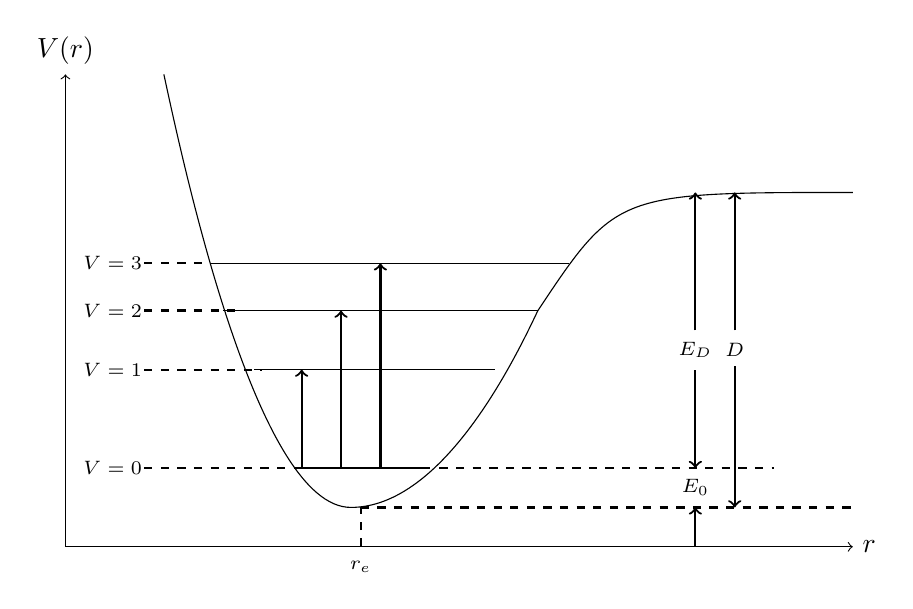
\begin{tikzpicture}
        \def\xmin{0}
        \def\xmax{10}
        \def\ymin{0}
        \def\ymax{6}

        (\xmax,\ymax);
        \draw[->] (\xmin,\ymin) -- (\xmax,\ymin) node[right] {$r$};
        \draw[->] (\xmin,\ymin) -- (\xmin,\ymax) node[above] {$V(r)$};

  \draw[] (1.25,6) parabola[parabola height=-4cm,very thick] bend (4.5,2) (6,3);
  \draw[] (6,3) .. controls (7,4.5) .. (10,4.5);

\node (v0) at (0.6,1) {\scriptsize $V = 0$};
\node (v1) at (0.6,2.25) {\scriptsize $ V = 1$};
\node (v2) at (0.6,3) {\scriptsize $ V = 2 $};
\node (v3) at (0.6,3.6) {\scriptsize $ V = 3$};

\draw[ thick, dashed]  (1,1) -- (3.125,1) ;
\draw[ thick, dashed]  (1,2.25) -- (2.5,2.25) ;
\draw[ thick, dashed]  (1,3) -- (2.25,3) ;
\draw[ thick, dashed]  (1,3.6) -- (1.75,3.6) ;

\draw[ thick, dashed]  (4.75,1) -- (9,1) ;
\draw[ thick, dashed]  (3.75,0.5) -- (10,0.5) ;

\draw[thick, dashed]  (3.75,0) -- (3.75,0.5) ;
\node (e0) at (8, 0.75) {\scriptsize $ E _0$};
\draw[->,thick]  (8,0) -- (8,0.5) ;

\draw[<-,thick]  (8,1) -- (8,2.25) ;
\node (ed) at (8, 2.5) {\scriptsize $ E _D$};
\draw[->,thick]  (8,2.75) -- (8,4.5) ;


\draw[<-,thick]  (8.5,0.5) -- (8.5,2.3) ;
\node (d) at (8.5, 2.5) {\scriptsize $ D$};
\draw[->,thick]  (8.5,2.75) -- (8.5,4.5) ;


\node (re) at (3.75, -0.25) {\scriptsize $ r _e$};

\draw[] (2.9,1) -- (4.625,1);
\draw[] (2.4,2.25) -- (5.45,2.25);
\draw[] (2,3) -- (6,3);
\draw[] (1.85,3.6) -- (6.4,3.6);

\draw[->, thick] (3,1) -- (3,2.25) ;
\draw[->, thick] (3.5,1) -- (3.5,3) ;
\draw[->, thick] (4,1) -- (4,3.6) ;


\end{tikzpicture}
}
\caption{Potenialverlauf für den anharmonischen Oszillator} \label{fig:M3}
\end{figure}

